\subsection{Recovery of the Schwarzschild Metric}
  \label{subsec:recovery-of-the-schwarzschild-metric}

  In the presence of a static and approximately spherically symmetric distribution of
  localized projected configurations, the collective reduction of admissible relaxation
  ordering admits a particularly simple effective description.
  In the weak-constraint and quasi-static regime, spatial variations of the effective
  ordering rate are governed by a Poisson-like relation linking an effective potential
  to the density of localized projected configurations.

  When a geometric parametrization becomes applicable, this structure is compactly
  summarized by an effective metric whose leading-order form coincides with the
  Schwarzschild solution of general relativity.
  In this description, the temporal component encodes the local reduction of admissible
  relaxation ordering (interpreted as gravitational time dilation), while the radial
  component reflects the corresponding modulation of correlation efficiency in the
  spatial sector.
  The angular part of the metric follows from the approximate isotropy of the projected
  configuration.

  Within this framework, the standard weak-field predictions of general relativity are
  recovered, including gravitational redshift, light deflection, and time dilation in
  agreement with solar-system observations.
  The gravitational constant \(G\) appears here as an emergent collective coupling
  parameter, relating the effective density of localized projected configurations to
  the magnitude of the admissible ordering slowdown.

  \begin{figure}[htbp]
    \centering
    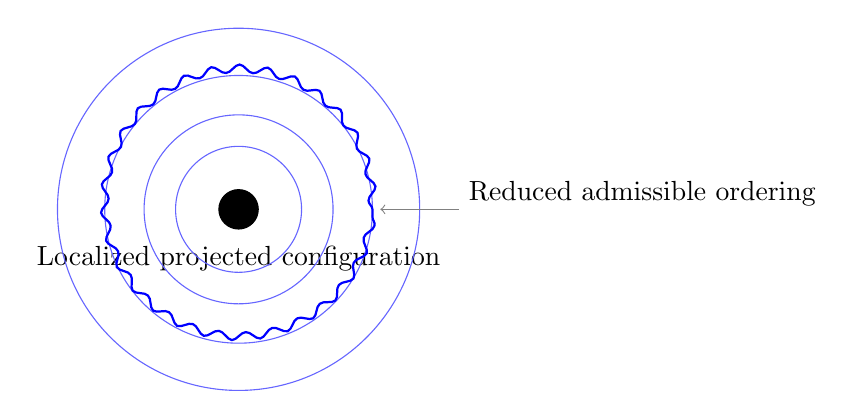
\begin{tikzpicture}[scale=1]

% Central mass
      \filldraw[black] (0,0) circle (0.25);
      \node[below] at (0,-0.35) {Localized projected configuration};

% Effective ordering contours
      \foreach \r in {0.8,1.2,1.7,2.3} {
        \draw[blue!60] (0,0) circle (\r);
      }

% Distortion
      \draw[blue, thick, decorate, decoration={snake, amplitude=0.5mm}]
      (0,0) circle (1.7);

% Arrows
      \draw[->, gray] (2.8,0) -- (1.8,0);
      \node[right] at (2.8,0.2) {Reduced admissible ordering};

    \end{tikzpicture}
    \caption
    {Emergence of Schwarzschild-like behavior in Cosmochrony.
    A localized projected configuration induces a spatially varying reduction of
    admissible relaxation ordering.
    In effective geometric descriptions, this manifests as differential proper-time
    accumulation and an emergent metric curvature analogous to gravitational time
    dilation.}
    \label{fig:chi_gravity}
  \end{figure}

  Importantly, the Schwarzschild metric is not postulated as a fundamental solution, nor
  is spacetime curvature treated as a primitive dynamical entity.
  The metric functions instead as a compact and operational summary of how localized
  projected configurations constrain admissible relaxation ordering in their vicinity.

  Schwarzschild-like behavior therefore does not reflect a specific dynamical law of
  spacetime itself.
  It emerges as the necessary phenomenological description in regimes where projected
  configurations are close to local equilibrium and admit a smooth geometric
  representation.
